% !TeX root = RJwrapper.tex
\title{Hdtg: An R Package for High-Dimensional Truncated Normal Simulation}
\author{by Zhenyu Zhang, Andrew Chin, Akihiko Nishimura and Marc A.~Suchard}

\maketitle

\abstract{
Simulating from the multivariate truncated normal distribution (MTN) is required in various statistical applications yet remains challenging in high dimensions.
Currently available algorithms and their implementations often fail when the number of parameters exceeds a few hundred.
To provide a general computational tool to efficiently sample from high-dimensional MTNs, we introduce the \CRANpkg{hdtg} package that implements two state-of-the-art simulation algorithms: harmonic Hamiltonian Monte Carlo (Harmonic-HMC) and zigzag Hamiltonian Monte Carlo (Zigzag-HMC).
Both algorithms exploit analytical solutions of the Hamiltonian dynamics under a quadratic potential energy with hard boundary constraints, leading to rejection-free methods.
We compare their efficiencies against another state-of-the-art algorithm for MTN simulation, the minimax tilting accept-reject sampler (MET).
The run-time of these three approaches heavily depends on the underlying multivariate normal correlation structure.
Zigzag-HMC and Harmonic-HMC both achieve 100 effective samples within 3,600 seconds across all tests with dimension ranging from 100 to 1,600, while MET has difficulty in several high-dimensional examples.
We provide guidance on how to choose an appropriate method for a given situation and illustrate the usage of \CRANpkg{hdtg}.
}

\section{Introduction}
Sampling from a multivariate truncated normal (MTN) distribution is a recurring problem in many statistical applications. 
The MTN distribution of a $ \dimd $-dimensional random vector $ \bm{x} \in \realNumbers^{\dimd}$ has the form   
	\begin{equation}
	\bm{x} \sim \normalDensityFunction{\mean}{\covariance} \text{ with } \left(\fmat\bposition + \gvec\right)_i \geq 0 \text{ for } i = 1, \dots, \numTruncs,
	\end{equation}
	where $ \mean $ and $ \covariance $ are the mean vector and covariance matrix, 		
	 the $ \numTruncs \times \dimd $ matrix $ \fmat $ and $ \numTruncs$-dimensional vector $ \gvec $ specify the $ \numTruncs $ linear constraints and $ \left(\cdot\right)_i $ denotes the $ i$th vector element \citep{pakman2014exact}.
MTNs arise in various contexts including probit and tobit models \citep{albert1993bayesian, tobin1958estimation}, latent Gaussian models \citep{bolin2015excursion}, copula regression \citep{pitt2006efficient}, spatial models \citep{tsionas2016spatial, baltagi2018generalized, zareifard2021heterogeneous}, Bayesian metabolic flux analysis \citep{heinonen2019bayesian}, and many others.
When the dimension $ \dimd $ is small, a standard rejection sampler \citep{geweke1991efficient, kotecha1999gibbs} works well and is a common choice.
However, simulation from a larger MTN with hundreds or thousands of correlated dimensions remains a computational challenge.
Work towards this goal includes harmonic Hamiltonian Monte Carlo \citep[\hhmc]{pakman2014exact}, rejection sampling based on minimax (saddle point) exponential tilting \citep[\mt]{botev2017normal}, and the most recent Zigzag Hamiltonian Monte Carlo \citep[\zhmc]{nishimura2020discontinuous, nishimura2024zigzag} methods.

The \mt method provides independent samples but can suffer from low acceptance rates and becomes impractical with $ \dimd > 100 $, except in special cases like when the MTN has a strongly positive correlation structure \citep{botev2017normal}.
Both \hhmc and \zhmc are Markov chain Monte Carlo (MCMC) approaches that generate correlated samples, but can nonetheless be highly efficient and scale to thousands or more dimensions.  
To our knowledge, however, there is no general-purpose implementation of either method;
the \pkg{tmg} package provided by \citet{pakman2014exact} is no longer available on CRAN, and \citet{zhang2023accelerating} implement \zhmc for their phylogenetics applications in the specialized software BEAST \citep{beast2018}. 
Therefore, we have developed the \CRANpkg{hdtg} R package for efficient  MTN simulation.
The package implements tuning-free \zhmc and \hhmc.
We provide performance comparisons among these two methods and a \mt implementation from the \CRANpkg{TruncatedNormal} package \citep{tnpkg}.
In most of the test cases with $ \dimd > 100 $, \hhmc and \zhmc outperform MET. 
We then conclude with some empirical guidance on which method to use in different scenarios.
\section{Algorithm}
\label{sec:algorithm}
We begin by briefly introducing \hhmc and \zhmc, both of which are variants of HMC, an effective proposal generation mechanism exploiting the properties of Hamiltonian dynamics \citep{hmcneal}.
\hhmc and \zhmc follow the same general framework.
To sample $ \bposition = \left(\position_1, \dots, \position_\dimd\right) \in \realNumbers^{\dimd}$ from the target distribution $ \positionDistribution{\bposition} $, the HMC variants introduce an auxiliary \textit{momentum} variable $ \bmomentum$ and define an augmented target distribution $\pi(\bposition, \bmomentum) = \positionDistribution{\bposition} \momentumDistribution{\bmomentum}$ in the joint space.
They then propose the next state by first re-sampling the momentum variable from its marginal and then simulating the solution of Hamiltonian dynamics governed by the differential equations
\begin{equation}
\label{eq:hamilton}
\frac{\diff \bposition}{\diff t}
= \nabla \kinetic(\bmomentum), \quad
\frac{\diff \bmomentum}{\diff t}
= - \nabla \potential(\bposition),
\end{equation}
where $\potential(\bposition)=- \log \positionDistribution{\bposition}$ and $\kinetic(\bmomentum) = - \log \momentumDistribution{\bmomentum}$ are referred to as \textit{potential} and \textit{kinetic} energies.
The dynamics are simulated for a pre-set time duration $\integrationTime$ and the end state constitutes a valid Metropolis proposal to be accepted or rejected according to the standard formula \citep{metropolis53, hastings1970monte}.

The most common versions of HMC use the momentum distribution $ \momentumDistribution{\bmomentum} \sim \mathcal{N}(\bm{0}, \M) $ and rely on the leapfrog integrator to numerically solve \eqref{eq:hamilton}, as its solutions are analytically intractable in general settings. \hhmc takes advantage of the fact that \eqref{eq:hamilton} admits analytical solutions when the target $\positionDistribution{\bposition}$ is an MTN.
The solution follows independent harmonic oscillations along the principal components of the covariance/precision matrix \citep{pakman2014exact};
we thus refer to the algorithm as \hhmc. 
Truncation boundaries are handled via elastic ``bounces'' against hard potential energy walls \citep{hmcneal}.
Algorithm \ref{alg:hhmc} provides pseudo-code for \hhmc following  \protect\citet{pakman2014exact}.

\zhmc differs from the common HMC versions in that it deploys a Laplace momentum  \citep{nishimura2020discontinuous, nishimura2024zigzag} 
	\begin{equation}
			\momentumDistribution{\bmomentum} \propto \prod_{i=1}^\dimd \exp\left(-|\momentum_i|\right).
	\end{equation}
The Hamiltonian dynamics then become
\begin{equation}
\label{eq:hzz_equation}
\frac{{\rm d} \bposition}{{\rm d} t}
=   \sign\left(\bmomentum\right), \quad
\frac{{\rm d} \bmomentum}{{\rm d} t} = - \nabla \potential(\bposition),
\end{equation}
where $\sign\left(\momentum_i\right)$ returns 1 if $\momentum_i$ is positive and -1 otherwise.
Because the velocity $\diff \bposition / \diff t \in \{\pm 1\}^\dimd$ remains constant until one of the $ \momentum_i $ flips its sign, the trajectory of these Hamiltonian dynamics has a zigzag pattern, hence the name \zhmc.
The zigzag dynamics also admit analytical solutions under an MTN target and can handle the truncation in the same manner as in \hhmc.
Algorithm \ref{alg:zhmc} provides pseudo-code for \zhmc. Our current \zhmc implementation is limited to the coordinate-wise bounds $\lb \leq \bm{x} \leq \ub$. We refer interested readers to \citet{nishimura2024zigzag} and \citet{zhang2023accelerating} for more details.

The simulation duration $\integrationTime$, i.e.\ how long Hamiltonian dynamics is simulated for each proposal generation, critically affects efficiencies of both Harmonic and Zigzag-HMC.
For \hhmc, \citet{pakman2014exact} suggest setting $ \integrationTime = \pi/2 $;
when using this fixed $ \integrationTime $, however, we observe inefficiencies in some of our examples in Section~\ref{sec:efficiency_comparison} due to Hamiltonian dynamics' periodic behaviors \citep{hmcneal}.
We therefore randomize the duration $\integrationTime$, as recommended by \citet{hmcneal}, and draw it from a uniform distribution on $ \left[\pi/8,\pi/2\right] $. 
For \zhmc, we adopt the choice $ \integrationTime =  \sqrt{2} \eigenvalue{\text{min}}^{-1/2}$ based on the heuristics of \cite{nishimura2024zigzag}, where $\eigenvalue{\text{min}} $ is the minimal eigenvalue of the precision matrix $ \precision = \covariance^{-1} $.
We compute $\eigenvalue{\text{min}} $ using the Lanczos algorithm \citep{demmel1997applied} as in the \CRANpkg{mgcv} package \citep{mgcvcite}.
We further implement the no-U-turn sampler (NUTS) of \citet{hoffman2014nuts} to automatically determine
the integration time. 
With NUTS, we only need to pick a base integration time $ \basestep $ which we set to $0.1 \eigenvalue{\text{min}}^{-1/2}$
as recommended by \citet{nishimura2024zigzag}.

	\singlespacing
	\begin{minipage}[t]{0.49\textwidth}
		\begin{algorithm}[H]
			\caption{\hhmc for MTNs}
			\label{alg:hhmc}
			\begin{algorithmic}[1]
				\REQUIRE $ \bposition, \integrationTime,  \bmu ,  \precision, \fmat, \gvec$, 

				\textbf{(1) Whitening:}
				\STATE \( R \gets \text{Cholesky}(\Omega) \)
				\STATE \( \bpositionwhitened \gets R(\bposition - \bmu) \)
				\spacersmall

				\textbf{(2) Momentum draw:}
				\STATE $ \bmomentum \sim \normalDensityFunction{\bzero}{\M} $
				\spacersmall

				\textbf{(3) Dynamics:}
				\STATE $ \tau \gets \integrationTime $ 
				\spacersmall

				\WHILE{$ \tau > 0 $}
				\spacersmall

				\STATE \% Find next boundary event
				\STATE $(\reflectTime, j_b) \gets \textsc{NextBounce}(\bpositionwhitened, \bmomentum, \fmat, \gvec)$
				\spacersmall

				\STATE \% The event time is bounded by $ \tau $
				\STATE $ \bounceTime \gets \min \{t_b, \tau\} $ 
				\spacersmall

				\STATE \% Advance time $ \bounceTime $: 
				\STATE $ \bpositionwhitened \gets \bmomentum \sin(\bounceTime) + \bpositionwhitened \cos(\bounceTime) $
				\STATE $ \bmomentum \gets \bmomentum \cos(\bounceTime) - \bpositionwhitened \sin(\bounceTime) $
				\spacersmall

				\STATE \% Update $ \bmomentum $ for a boundary event
				\STATE \% $ \fmat_{j_b} $ is the $ j_b $th row vector of $ \fmat $
				\IF{$t < \tau$}
				\STATE $\alpha \gets \dfrac{\fmat_{j_b} \cdot \bmomentum}{\fmat_{j_b} \cdot \fmat_{j_b}}$
				\STATE $\bmomentum \gets \bmomentum - 2\alpha \fmat_{j_b}^\top$
				\ENDIF

				\STATE $ \tau \gets \tau - \bounceTime $
				\spacersmall

				\ENDWHILE
				\spacersmall

				\textbf{(4) Unwhiten:}
				\STATE $ \bposition \gets R^{-1}\bpositionwhitened + \bmu $
				\RETURN $ \bposition $
				\spacersmall

				\textbf{Function} \textsc{NextBounce}($ \bpositionwhitened, \bmomentum, \fmat, \gvec $):
				\STATE $t_{\text{b}} \gets \infty$, $j_{\text{b}} \gets -1$
				\spacersmall

				\FOR{$j = 1$ \textbf{to} $m$}
				\STATE \% $ (\fmat \bmomentum)_j $ is the $j$th element of $ \fmat \bmomentum $
				\STATE $f_a \gets  (\fmat \bmomentum)_j$, $f_b \gets  (\fmat \bpositionwhitened)_j$
				\spacersmall
				\STATE $u_j \gets \sqrt{f_a^2 + f_b^2}$
				\spacersmall

				\IF{$u_j > |g_j|$}
				\STATE $\varphi_j \gets -\operatorname{atan2}(f_a, f_b)$
				\STATE $A \gets \arccos(-g_j/u_j)$
				\STATE $t_1 \gets -\varphi_j + A$
				\STATE $t_2 \gets -\varphi_j - A + 2\pi$
				\IF{$t_1 < 0$}
				\STATE $ t_{\text{c}} \gets t_2 $
				\ELSE \STATE $t_{\text{c}} \gets \min(t_1, t_2)$
				\ENDIF
				\spacersmall

				\IF{$t_{\text{c}} < t_{\text{b}}$}
				\STATE $t_{\text{b}} \gets t_{\text{c}}$, $j_{\text{b}} \gets j$
				\ENDIF
				\ENDIF
				\ENDFOR
				\spacersmall

				\RETURN $(t_{\text{b}}, j_{\text{b}})$

			\end{algorithmic}
		\end{algorithm}
	\end{minipage}
	\hfill
	\begin{minipage}[t]{0.49\textwidth}
		\begin{algorithm}[H]
			\caption{\zhmc for MTNs}
			\label{alg:zhmc}
			\begin{algorithmic}[1]
				\REQUIRE $\bposition$, \integrationTime, $ \bmu $, $ \precision $

				\textbf{(1) Momentum draw:} \\
				\STATE $ \momentum_i \sim \operatorname{Laplace}(u=0, b=1)$ 
				\STATE $ \bvelocity \gets \operatorname{sign}(\bmomentum) $ 
				\spacersmall

				\textbf{(2) Pre-compute:} \\
				\STATE $\bm{\varphi}_{\bposition} \gets \precision (\bposition - \bmu)$ 
				\STATE $\bm{\varphi}_{\bvelocity} \gets \precision \bvelocity$ 
				\spacersmall

				\textbf{(3) Dynamics:} \\
				\STATE $ \tau \gets \integrationTime $ 
				\spacersmall

				%\STATE \textbf{while} $ \tau > 0 $ \textbf{do} \\
				\WHILE{$ \tau > 0 $}
				\spacersmall
				\STATE \% Find gradient event time $ \gradientTime $ 
				\STATE $ \ba \gets  \bm{\varphi}_{\bvelocity} /2, \bb \gets \bm{\varphi}_{\bposition}, \bc \gets -\bmomentum$
				\STATE $ \gradientTime \gets \min_i \{\text{minPositiveRoot}(a_i, b_i, c_i) \}^*$

				\spacersmall
				\STATE \%Find boundary event time $ \reflectTime $ 
				\FOR{$i = 1$ \TO $\dimd$}
				\IF{$\velocity_i > 0$}
				\STATE $t_i \gets U_i - \position_i$
				\ELSE
				\STATE $t_i \gets \position_i - L_i$
				\ENDIF
				\ENDFOR
				\STATE	$ \reflectTime \gets  \min_i t_i$
				\spacersmall
				\STATE \%The actual event happens at time $ \bounceTime $ 
				\STATE $ \bounceTime \gets \min \{ \gradientTime, \reflectTime, \tau\}  $
				\spacersmall

				\STATE{\% Advance time $ \bounceTime $} 
				\STATE $ \bposition \gets \bposition +  \bounceTime \bvelocity$ 
				\STATE $ \bmomentum \gets \bmomentum - \bounceTime \phix - \bounceTime^2 \phiv / 2$ 
				\STATE $ \phix \gets \phix + \bounceTime \phiv $ \\
				\spacersmall
				\STATE{\% Update momentum} 
				\IF{a gradient event happens at $ i_g $}
				\STATE $\velocity_{i_g} \gets -\velocity_{i_g}$  

				\ELSIF{a boundary event happens at $ i_b $}
				\STATE $\velocity_{i_\textrm{b}} \gets -\velocity_{i_\textrm{b}}$, $\momentum_{i_\textrm{b}} \gets -\momentum_{i_\textrm{b}}$ 
				\ENDIF
				\spacersmall

				\STATE $ \phiv \gets \phiv + 2\velocity_i \precision \basisVector_i $
				\STATE{\% $ \basisVector_i  $ has 1 in position $ i $ and 0 elsewhere}
				\STATE $ \tau \gets \tau - \bounceTime $

				\ENDWHILE
				\RETURN $ \bposition $
			\end{algorithmic}
			*$\text{minPositiveRoot}(a_i, b_i, c_i) $ returns the minimal positive root of the equation $ a_i t^2 + b_i t + c_i = 0 $, or returns $+\infty$ if no positive root exists.
		\end{algorithm}
	\end{minipage}

The algorithmic divergence between the two methods stems from their momentum distributions. \hhmc employs Gaussian momentum, generating harmonic oscillatory dynamics via trigonometric functions. In contrast, \zhmc uses Laplace momentum, producing piecewise-linear trajectories with constant velocity updates. This distinction leads to differences in event detection: \hhmc computes boundary bounce times using trigonometric relationships, while \zhmc solves quadratic equations for gradient events and checks coordinate distances for boundary events (Algorithm \ref{alg:hhmc} and \ref{alg:zhmc} ). These algorithmic differences lead to varying opportunities for implementation optimization, as summarized in Table \ref{tab:implementation-comparison}. The piecewise-linear dynamics of \zhmc, consisting primarily of vector additions and multiplications, map well to single instruction multiple data (SIMD) instructions, which can process multiple values simultaneously within a single CPU core. In contrast, \hhmc's trigonometric operations (sin, cos, atan2, arccos) are inherently less SIMD-friendly due to their transcendental nature. While both samplers are implemented in optimized C++ with Eigen for linear algebra, \zhmc's algorithmic structure is inherently more amenable to the low-level hardware optimizations (SIMD and aligned memory) that yield performance gains on modern processors. When examining the computational performance benchmarks in Section~\ref{sec:efficiency_comparison}, it is important to recognize that the observed speed differences stem from both algorithmic efficiencies and the hardware-specific optimizations detailed here.

\tbCompare

In addition to \hhmc and \zhmc, the \CRANpkg{hdtg} package also implements the \mzz sampler \citep{bierkens2019ergodicity} for MTNs. The \mzz belongs to another emerging class of MCMC algorithms that are based on piecewise deterministic Markov processes (PDMP) \citep{fearnhead2018piecewise}. As established by \cite{nishimura2024zigzag}, \mzz is a close cousin of the Hamiltonian-based \zhmc, with the key difference being the amount of retained momentum information during sampling. \mzz exhibited lower sampling efficiency compared to \hhmc and \zhmc, particularly on targets with correlated parameters \citep{nishimura2024zigzag}. Therefore, we do not include \mzz in our performance comparisons of Section \ref{sec:efficiency_comparison}. The \mzz function is nevertheless available in the package for users who wish to experiment with it.

\section{Using hdtg}\label{sec:pkg}
The \CRANpkg{hdtg} package allows users to draw MCMC samples from an MTN.
As an example, one may use the following code to generate 1,000 samples from a 10-dimensional MTN with zero mean and an identity covariance matrix truncated to the positive orthant:

\begin{example}
# set the random seed
set.seed(1)
# draw MTN samples using Zigzag-HMC 
samplesZHMC <- zigzagHMC(nSample = 1000, mean = rep(0, 10), prec = diag(10), 
                         init = rep(0.1, 10), lowerBounds = rep(0, 10), 
                         upperBounds = rep(Inf, 10))
# draw MTN samples using Harmonic-HMC 
samplesHHMC <- harmonicHMC(nSample = 1000, mean = rep(0, 10), choleskyFactor = diag(10),
		           precFlg = TRUE, init = rep(0.1, 10), 
		           constrainDirec = diag(10), constrainBound = rep(0, 10))
\end{example}
The arguments are:
\begin{itemize}
	\item \code{nSample}: number of samples.
	\item \code{mean}: a $ \dimd $-dimensional mean vector.
	\item \code{prec}: the precision matrix.
	\item \code{init}: a vector of the initial value that must satisfy all constraints.
	\item \code{lowerBounds}: a $ \dimd $-dimensional vector specifying the lower bounds.
	\item \code{upperBounds}: a $ \dimd $-dimensional vector specifying the upper bounds.
	\item \code{choleskyFactor}: upper triangular matrix $ \umat $ from Cholesky decomposition of precision or covariance matrix into $ \umat\transpose\umat $.
	\item \code{precFlg}: whether \code{choleskyFactor} is from precision (\code{TRUE}) or covariance matrix (\code{FALSE}).
	\item \code{constrainDirec}: the $ \fmat $ matrix.
	\item \code{constrainBound}: the $ \gvec $ vector.

\end{itemize}
In addition to applications with fixed $\mean$ and $\precision$, hierarchical modeling may require sampling these parameters from their respective conditional distributions, such as the phylogenetics example \citep{zhang2023accelerating} where their posterior distributions are of scientific interest. In such ``random $\mean$ or $\precision$'' settings, one may call \code{zigzagHMC} or \code{harmonicHMC} inside an MCMC loop, with $\mean$ and $\precision$ updated at each iteration. For \zhmc, a more efficient approach is to reuse the existing C\texttt{++} engine object which already stores the truncation boundaries and SIMD configuration and simply pass the updated $\mean$ and $\precision$ to the sampler. The example below illustrates the 10-dimensional MTN case with a random mean and precision. Note that the stationary distribution of this toy example is the joint distribution of both the MTN parameters (\code{m}, \code{prec}) and the truncated MTN variable itself. While the conditional distributions are standard (normal for \code{m}, Wishart for \code{prec}, MTN for the variable), their joint distribution is not a standard named distribution and does not admit a closed-form expression.
\begin{example}
set.seed(1)
n <- 1000 
d <- 10
samples <- array(0, c(n, d))
# initialize MTN mean and precision
m <- rnorm(d, 0, 1)
prec <- rWishart(n = 1, df = d, Sigma = diag(d))[,,1]

# call createEngine once
engine <- createEngine(dimension = d, lowerBounds = rep(0, d),
upperBounds = rep(Inf, d), seed = 1, mean = m, precision = prec)

HZZtime <- sqrt(2) / sqrt(min(mgcv::slanczos(A = prec, k = 1, 
			  kl = 1)[['values']]))

currentSample <- rep(0.1, d)
for (i in 1:n) {
   m <- rnorm(d, 0, 1)
   prec <- rWishart(n = 1, df = d, Sigma = diag(d))[,,1]
   setMean(engine = engine, mean = m)
   setPrecision(engine = engine, precision = prec)
   currentSample <- getZigzagSample(position = currentSample, nutsFlg = F,
	   		         engine = engine, stepSize = HZZtime)
   samples[i, ] <- currentSample
}
\end{example}

\section{Efficiency comparison and method choice}
\label{sec:efficiency_comparison}
To assess the performance of \hhmc, \zhmc and \mt, we compare them on MTNs with a variety of correlation structures. 
The three examples are: 1) MTNs with its covariance matrix $ \covariance $ drawn from the uniform LKJ distribution \citep{lewandowski2009generating} as implemented in the \code{rlkjcorr} function from package \CRANpkg{trialr} \citep{trialrpkg};
2) MTNs with a compound symmetric covariance matrix such that $ \covariance_{i,i} = 1 $ and $ \covariance_{i,j} =  0.9 $ for $ i \neq j $; and
3) a real-world MTN that arises as a posterior conditional distribution in a statistical phylogenetics model of HIV evolution \citep{zhang2021large, zhang2023accelerating}.
For simplicity, we assume the truncation $ x_i > 0 $ for $ i = 1, \dots, \dimd$ in the first two examples.
For the HIV example, the truncation is determined by the signs of observed binary biological features.

We now specify our comparison criteria and the rationale behind them.
A more efficient MCMC algorithm takes shorter time to achieve a certain effective sample size (ESS).
For all three samplers considered, we compare their run-time to obtain the first 1, 100, or 1000 effectively independent samples ($\timeFirstSample, \timeHundredSamples, \timeKiloSamples $).
We include all three metrics because $\timeHundredSamples $ and $\timeKiloSamples $ reflect a practical run-time for simulation from a fixed MTN and $ \timeFirstSample $ better captures the pre-processing overhead that remains relevant in cases where $\covariance$ is random. 
Recall that the main pre-processing costs are the Cholesky decomposition of $ \covariance $ or $ \precision $ (\hhmc), calculating the minimal precision matrix eigenvalue $ \eigenvalue{\text{min}} $ (\zhmc), and solving the minimax optimization problem (\mt).
Therefore we have 
\begin{equation}\label{eq:time}
\begin{split}
\timeFirstSample & = \timePre + \timeIter, \\
\timeHundredSamples & =  \timePre + 100\timeIter, \\
\text{and } \timeKiloSamples & =  \timePre + 1000\timeIter, 
\end{split}
\end{equation}
where $ \timePre $ and $ \timeIter $ are the pre-processing time required for each $ \covariance $ update and the average run-time per one effective sample.
For simulation from a fixed MTN, $ \timePre $ is a one-time cost and so $ \timeHundredSamples $ or $\timeKiloSamples$ serve as better efficiency criteria.
When $ \cov $ is random (e.g.\ the second example in Section \ref{sec:pkg}), if $ \cov $ changes its value $ k $ times, the total run-time to obtain one effective sample for each $ \cov $ is $ k \timeFirstSample $ and so the $ \timeFirstSample $ criterion would be more informative.

For \hhmc and \zhmc, we estimate the ESS using the \CRANpkg{coda} package \citep{codapkg} and define $ \nsample $ as the average number of MCMC iterations required for one effectively independent sample.
We approximate $ \nsample $ by $ \chainLength / \text{ESS}_{\text{min}}$, where $\text{ESS}_{\text{min}}$ is the minimal ESS across all dimensions and $\chainLength $ is the chain length. 
We fix $ \nsample = 1$ for \mt as it generates independent samples.
Therefore $ \timeIter $ in Equation \eqref{eq:time} equals the average time to complete $ \nsample $ iterations after pre-processing.
Table \ref{tb:All} reports our efficiency comparison in terms of $\timeFirstSample$, $\timeHundredSamples $, and $ \timeKiloSamples $.
We run each test on an Apple M1 Pro equipped machine with 16GB of memory. Code and data to reproduce the results are available on Zenodo at \url{https://doi.org/10.5281/zenodo.18618209}.

\tbAll

The efficiency of all three methods strongly depends on the correlation structure.
\mt fails to generate 100 effectively independent samples within two hours in a few higher dimensional tests, while \hhmc and \zhn enjoy a $ \timeHundredSamples < 3600$ seconds across all tests.
In the LKJ example, \zhn achieves comparable performance to \hhmc when $ \dimd$ reaches $400$. For high-dimensional LKJ and HIV ($\dimd = 1600$) tests, \zhmc outperforms competing methods. \znuts is no more efficient than \zhmc across the tested examples.
On the other hand, when $ \covariance $ is compound symmetric with a high correlation of 0.9, \hhmc consistently outperforms the other methods.
For \mt, since solving the initial minimax optimization dominates its run-time, the cost scales sub-linearly with sample count ($ \timeHundredSamples < 100\timeFirstSample $ and $ \timeKiloSamples  < 1000\timeFirstSample $). This makes \mt the preferred method when many effective samples are desired (as in HIV $ \dimd=100,400 $ examples).

\begin{figure}[htbp]
	\centering
	% First row: MTN A and MTN B
	\begin{subfigure}[b]{0.48\textwidth}
		\centering
		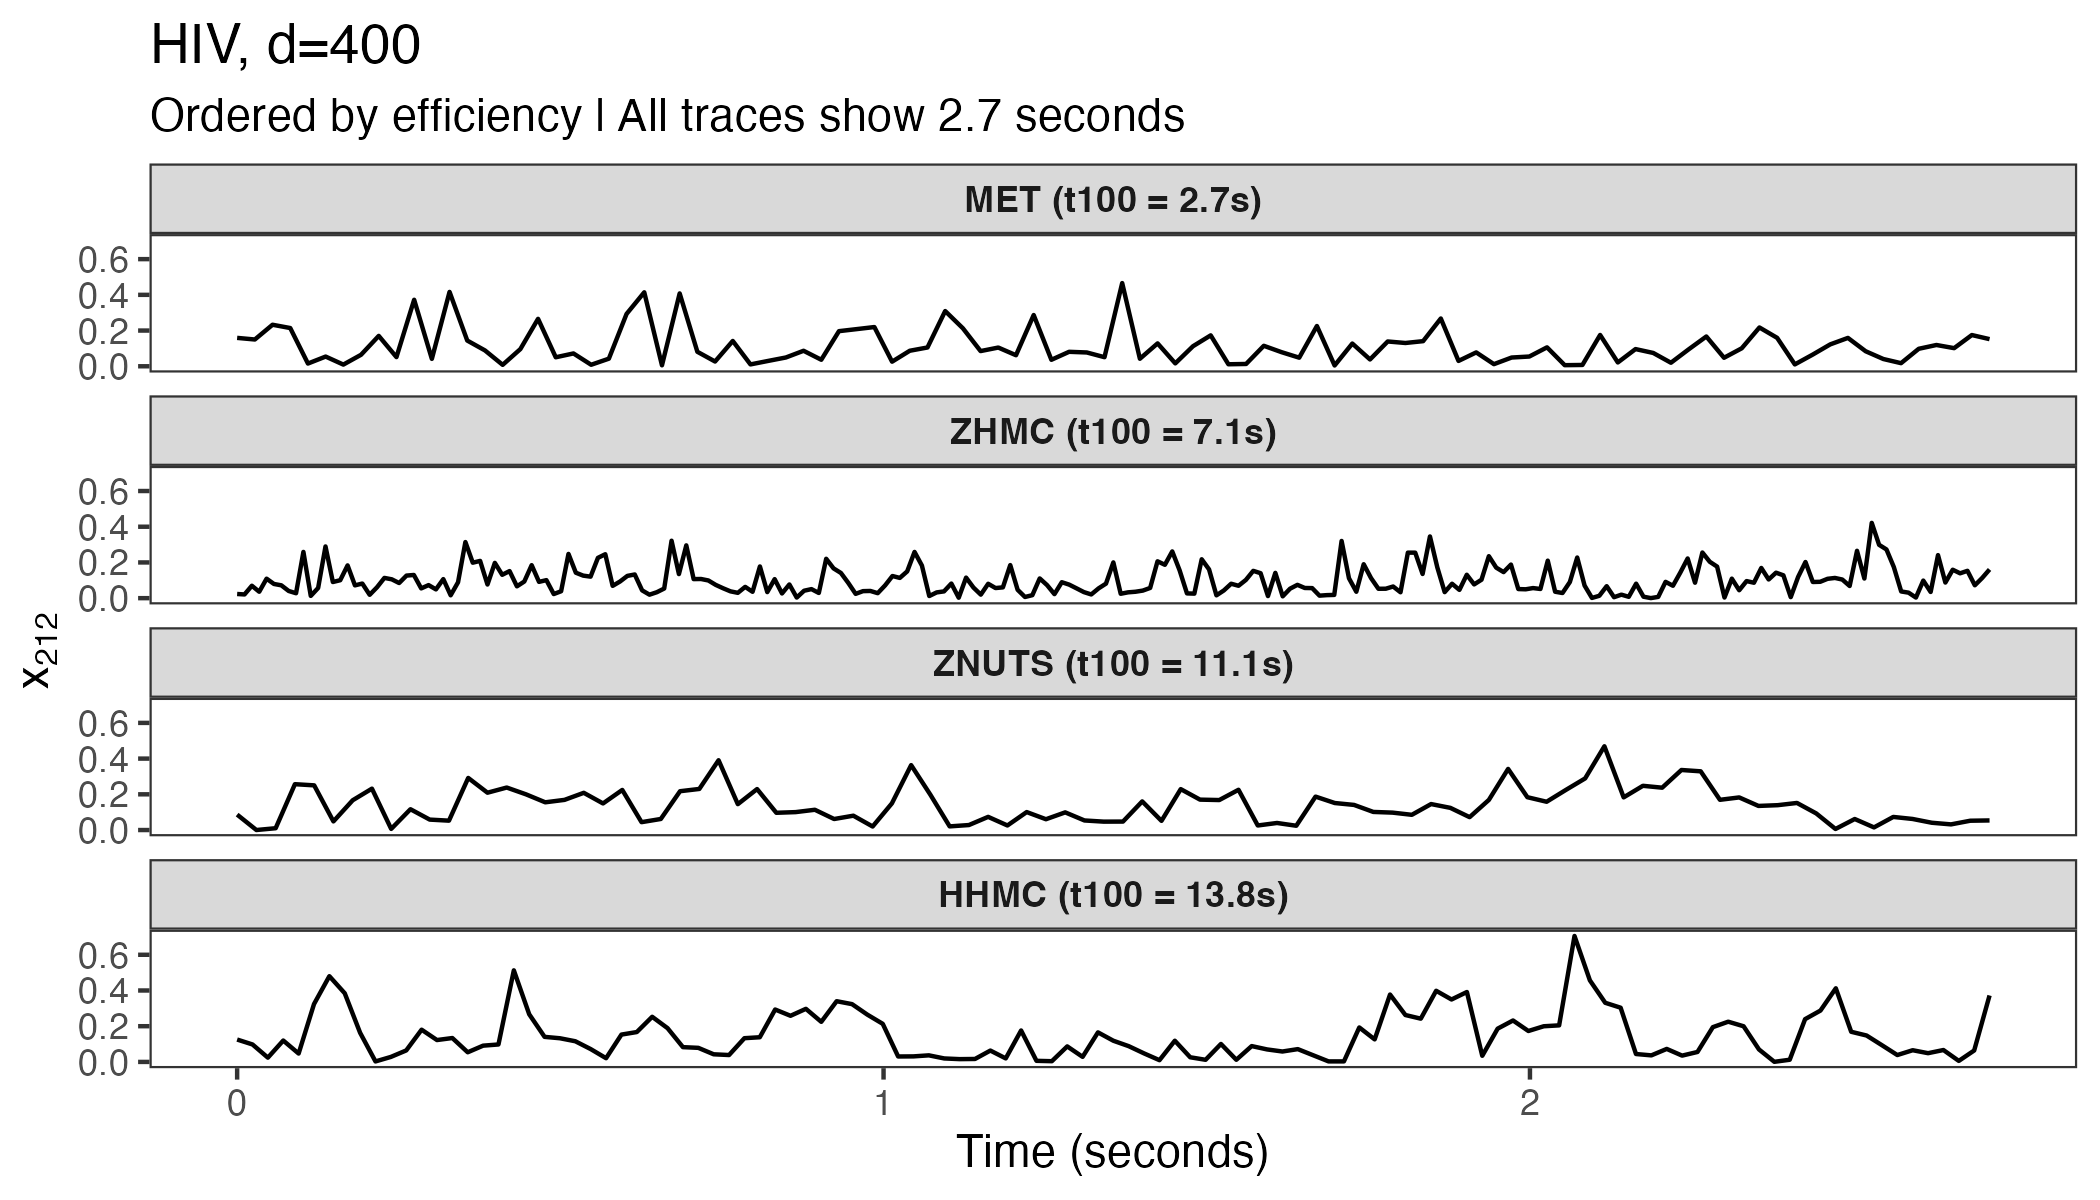
\includegraphics[width=\textwidth]{figures/time_normalized_HIV_d400.png}
		\caption{HIV, $ \dimd = 400 $}
		\label{fig:sub1}
	\end{subfigure}
	\hfill
	\begin{subfigure}[b]{0.48\textwidth}
		\centering
		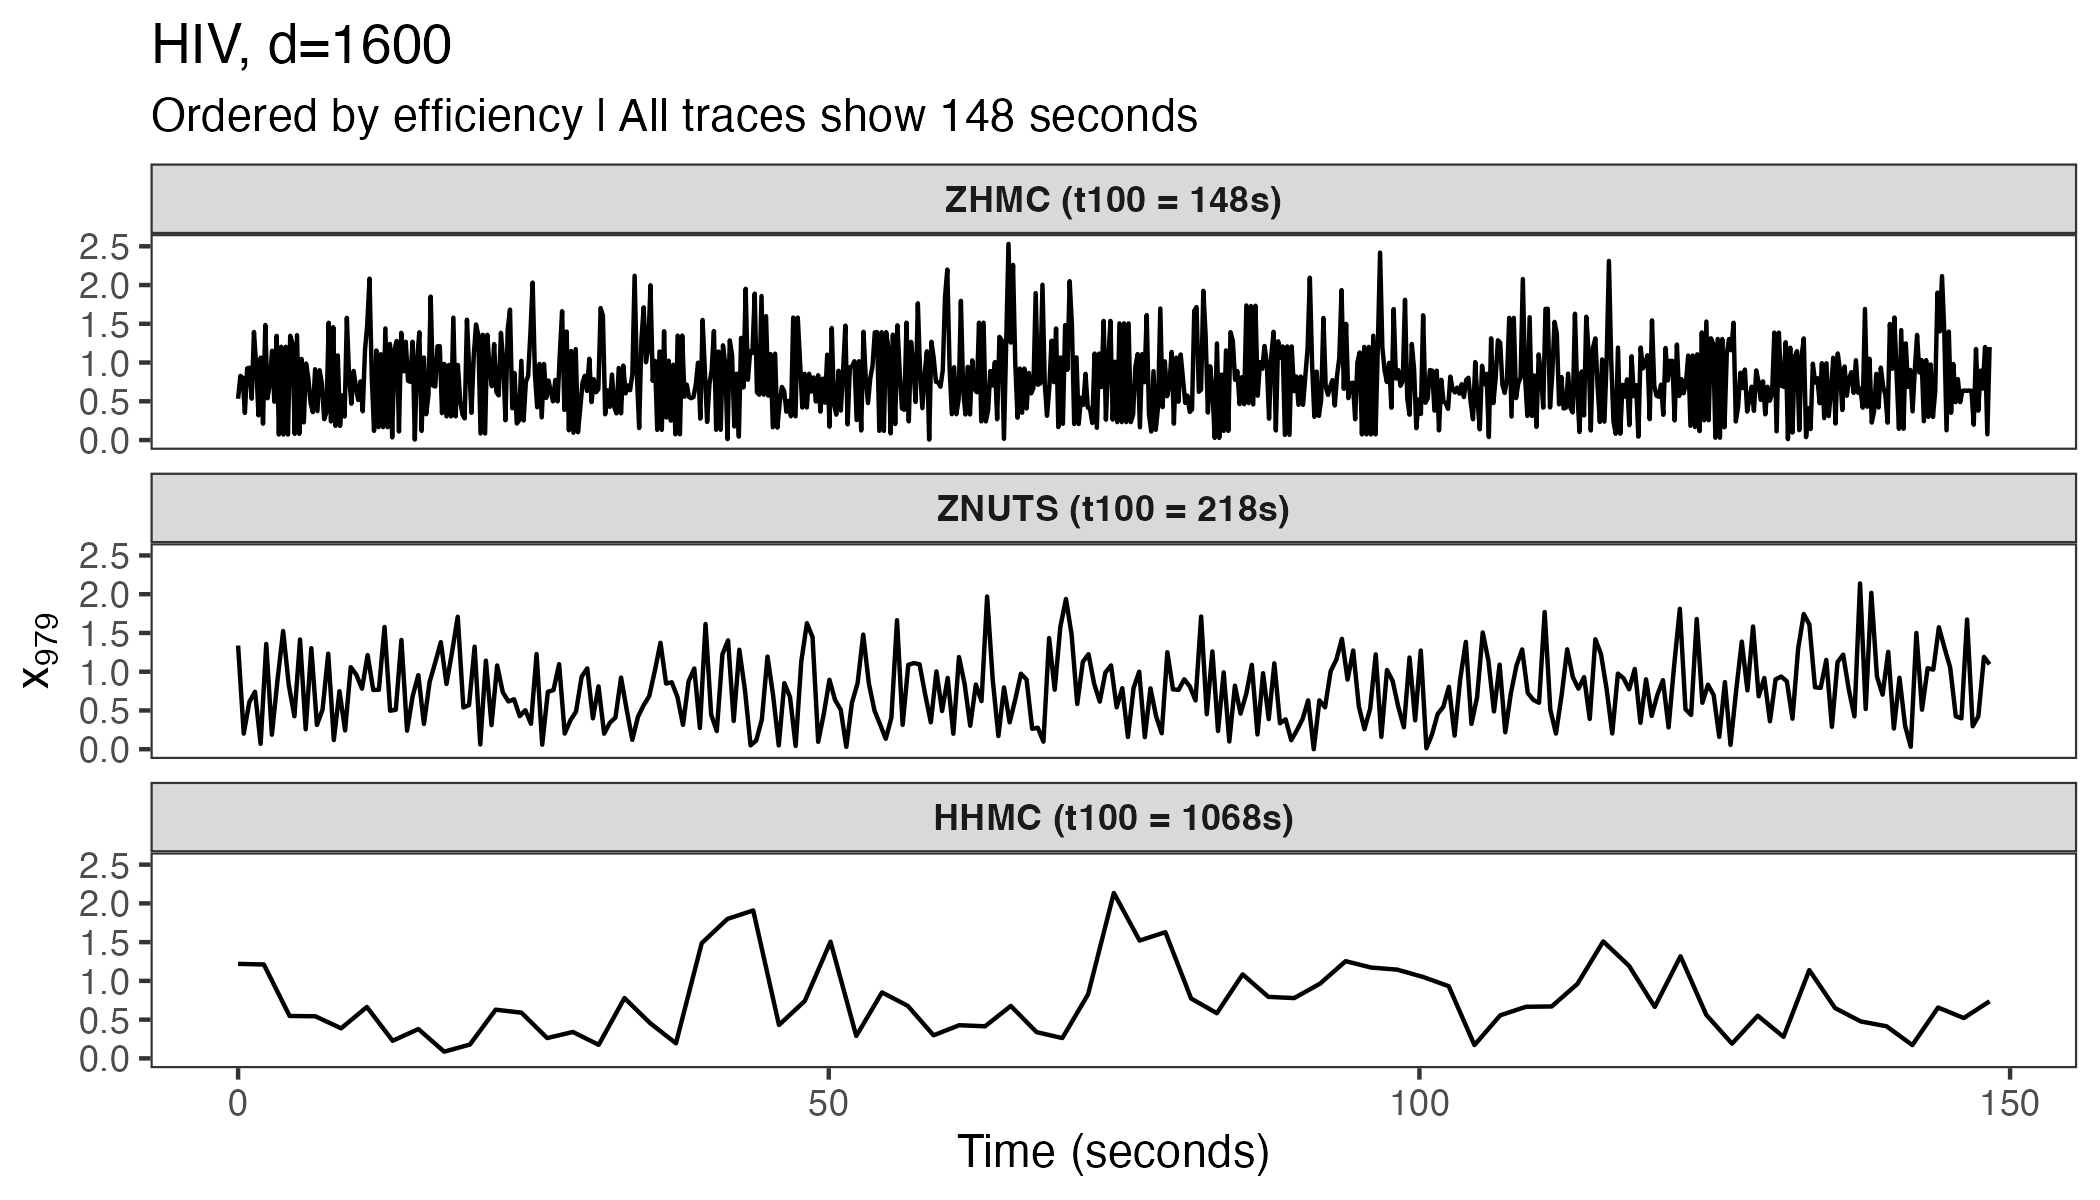
\includegraphics[width=\textwidth]{figures/time_normalized_HIV_d1600.png}
		\caption{HIV, $ \dimd = 1600 $}
		\label{fig:sub2}
	\end{subfigure}

	\vspace{0.5cm}

	% Second row: MTN C and MTN D
	\begin{subfigure}[b]{0.48\textwidth}
		\centering
		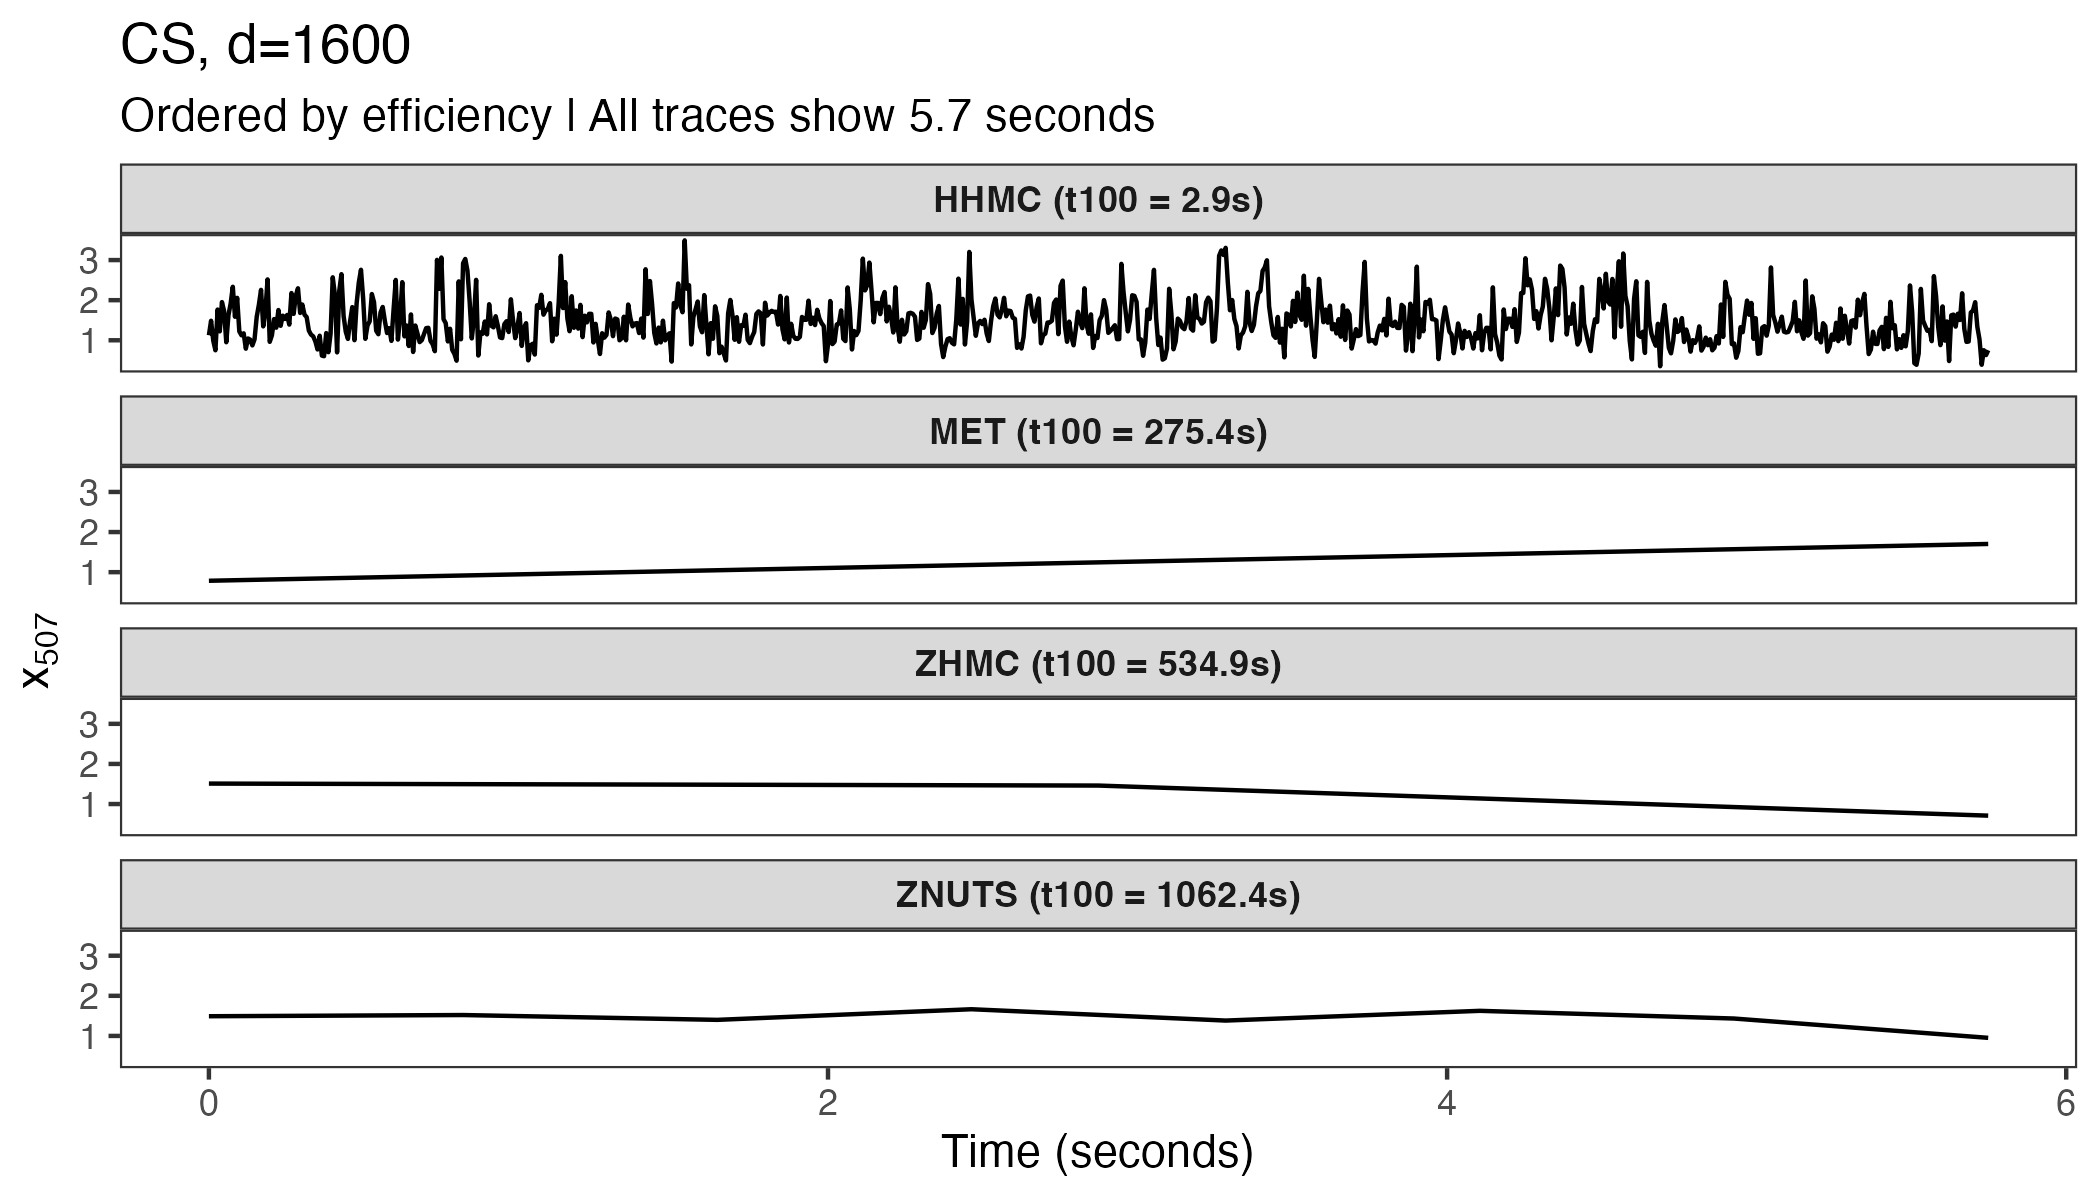
\includegraphics[width=\textwidth]{figures/time_normalized_CS_d1600.png}
		\caption{CS, $ \dimd = 1600 $}
		\label{fig:sub3}
	\end{subfigure}
	\hfill
	\begin{subfigure}[b]{0.48\textwidth}
		\centering
		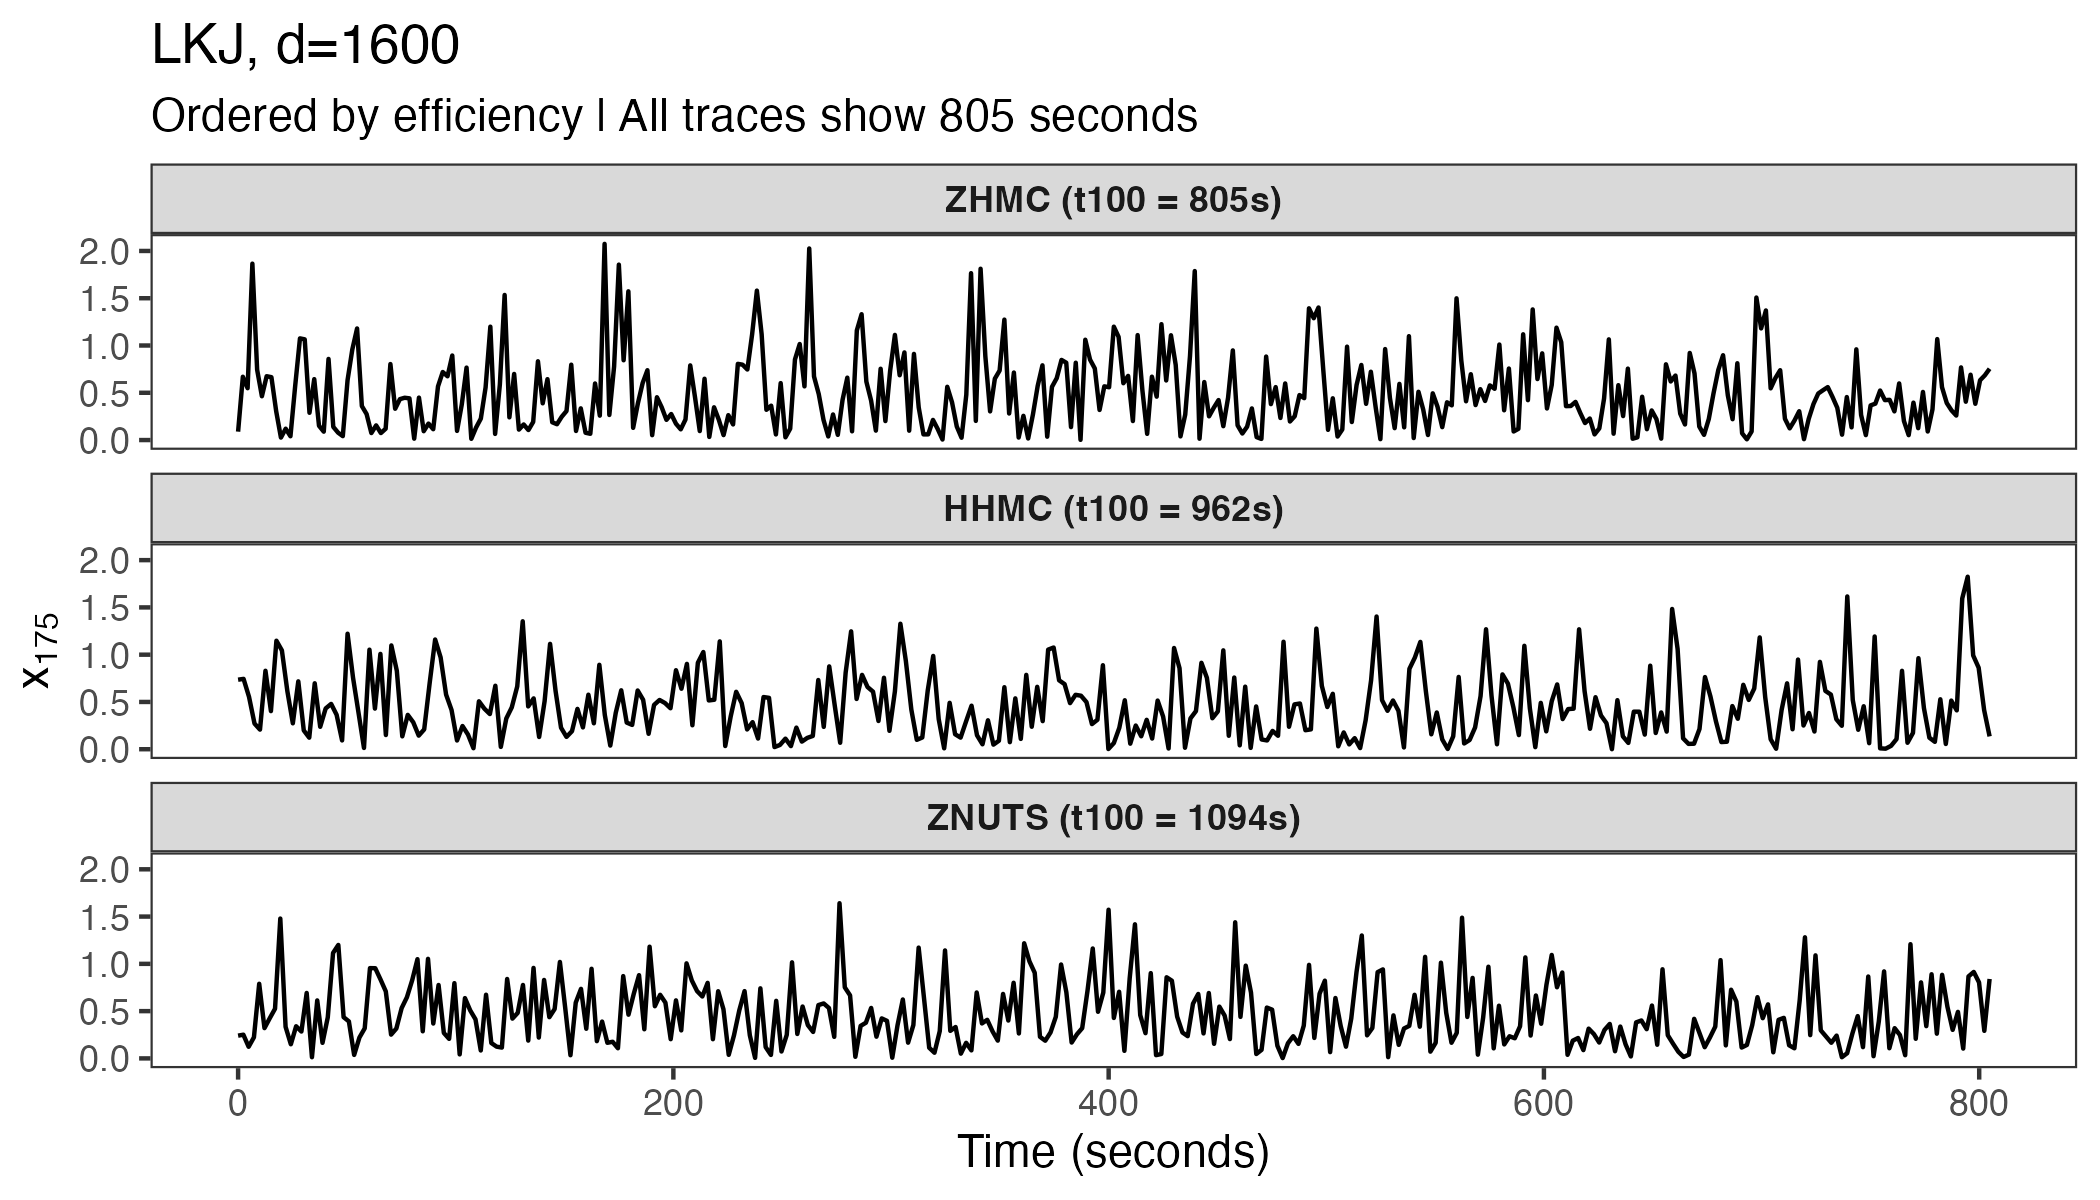
\includegraphics[width=\textwidth]{figures/time_normalized_LKJ_d1600.png}
		\caption{LKJ, $ \dimd = 1600 $}
		\label{fig:sub4}
	\end{subfigure}

	\caption{Time-normalized traceplots for four target MTNs using \CRANpkg{ggplot2} \citep{ggplot}. The y-axis shows a randomly selected dimension.}
	\label{fig:traceplots_all}
\end{figure}

Figure~\ref{fig:traceplots_all} shows traceplots for four target MTNs from Table~\ref{tb:All}. Different methods excel on different targets, highlighting the importance of target-specific algorithm selection. In practice, we recommend running a quick efficiency comparison to decide which method to use.
Nevertheless we provide some general guidance on method choice for high-dimensional MTN simulation:
\begin{itemize}
	\item If $ \dimd \leq 100 $ or the correlation structure is strongly positive, use \mt or \hhmc. 
	\hhmc may run faster but \mt has the advantage of generating independent samples.
	\item For $ \dimd > 1000$,  \zhn is presumably more efficient, though \hhmc may still outperform under strongly positive correlations. 
	\item It is always worth trying \mt which is free of MCMC convergence concerns. Since our simulation only examines a few correlation structures, it is possible that \mt can handle other large MTNs. 
\end{itemize}
A final point that needs consideration is that \zhn requires $ \precision $ and if only $ \covariance $ is available, the method first inverts $ \covariance $. This is a one-time operation and likely negligible cost when $ \covariance $ is constant. 
The approach does become expensive if $ \covariance $ is random, as the $ \order{\dimd^3} $ inversion is necessary for each value of $ \covariance $.
In practice, statistical models may be parameterized in terms of  $ \covariance $  \citep{lachaab2006modeling, molstad2021gaussian} or $ \precision $ \citep{baltagi2018generalized, lehnert2019large, li2020using}.
\hhmc carries a similar limitation since it requires a $ \order{\dimd^3} $ Cholesky decomposition of $ \covariance $ or $ \precision $, whichever is provided.
Therefore, when $ \dimd $ is large and the target MTN has a random correlation structure, one may favor \zhn over \hhmc especially if a closed-form $ \precision $ is at hand.

\section{Conclusion}
\SetSinglespace{1}
This article introduces the \CRANpkg{hdtg} package oriented for efficient MTN simulation.
In most of our high-dimensional tests the implemented \hhmc and \zhmc algorithms outperform the current best approach available in the \CRANpkg{TruncatedNormal} package.
To our best knowledge, \CRANpkg{hdtg} is the first tool that can generate samples from an arbitrary MTN with thousands of dimensions. 
We discuss the usage of functions and provide practical suggestions on method choice.
We expect to see future large-scale statistical applications utilizing the efficiency of \CRANpkg{hdtg}.

\section{Acknowledgment}
The \CRANpkg{hdtg} package itself leverages several R infrastructure packages including \CRANpkg{Rcpp} \citep{rcpppkg}, \CRANpkg{RcppEigen} \citep{eigenpkg}, \CRANpkg{RcppParallel}\citep{parallelpkg}, and \CRANpkg{mgcv} \citep{mgcvcite} for efficient computation. It also incorporates external header-only libraries: \texttt{sse2neon.h} \citep{sse2neon2020} for ARM support and \texttt{span.h} \citep{span2020} for memory-safe array views.
Research reported in this publication was supported by the National Institute of General Medical Sciences and the National Institute of Allergy and Infectious Diseases of the National Institutes of Health under award numbers  R35GM160458 (A.N.) and R01AI153044 (M.S.). The content is solely the responsibility of the authors and does not necessarily represent the official views of the National Institutes of Health."

\bibliography{hzz_rjournal}

\address{Zhenyu Zhang\\
  Department of Biostatistics, Fielding School of Public Health,\\
  University of California, Los Angeles, \\
  650 Charles E. Young Dr. South, Los Angeles, CA\\
  USA\\
  ORCiD: 0000-0002-2176-2253\\
  \email{zyz606@ucla.edu}}

\address{Andrew Chin\\
  Department of Biostatistics, Bloomberg School of Public Health,\\
  Johns Hopkins University,\\
 615 North Wolfe Street, Baltimore, MD 21205\\
 USA\\
 ORCiD: 0009-0005-3832-841X\\
  \email{achin23@jhu.edu}}

\address{Akihiko Nishimura \\
  Department of Biostatistics, Bloomberg School of Public Health,\\
  Johns Hopkins University,\\
  615 North Wolfe Street, Baltimore, MD 21205\\
  USA\\
  ORCiD: 0000-0002-6932-2513\\
  \email{aki.nishimura@jhu.edu}}

\address{Marc A.~Suchard\\
	Department of Human Genetics, David Geffen School of Medicine,\\
	Department of Biomathematics, David Geffen School of Medicine,\\
	Department of Biostatistics, Fielding School of Public Health,\\
	University of California, Los Angeles,\\
	695 Charles E. Young Drive, South, Los Angeles, CA\\
	USA\\
	ORCiD: 0000-0001-9818-479X\\
	\email{msuchard@ucla.edu}}
